\noindent
\section{Profiling Anomalous Reviewers}
\label{profile}


In this section we analyze in more details the performance of the anomalous reviewers. To this aim, we consider for each reviewer, the sequence of papers accepted by her and the citation accrued (within the first three years from publication) by each of these papers. A decreasing trend would suggest decline in performance of the reviewer. Depending on the trend we observe three broad categories within the set of anomalous reviewers \\
(i) performance deteriorates constantly over time (proportion = $42.5\%$, figure \ref{cit_prof}(a)).\\
(ii) performance is good for initial few papers but deteriorates in the long run (proportion = $22.6\%$, figure \ref{cit_prof}(b)).\\
(iii) performance fluctuates but has a deteriorating trend in the long run (proportion = $34.9\%$, figure \ref{cit_prof}(c)).
\begin{figure}
\centering
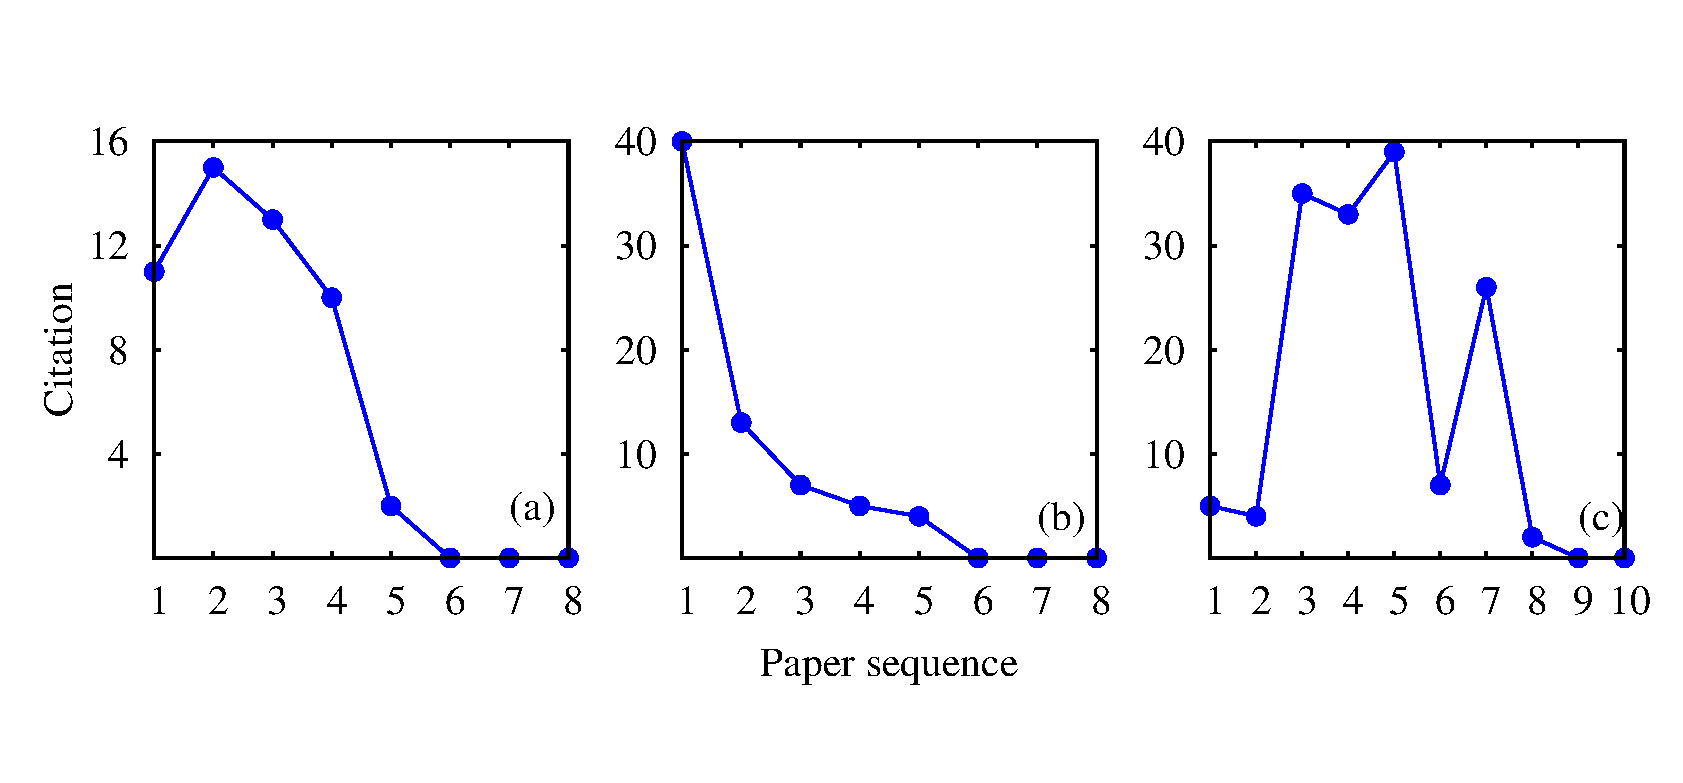
\includegraphics[scale=0.3]{figures/profile_all.eps}
\caption{\label{cit_prof} Mean citation profile of the reviewers in the three categories.}
\vspace{-.4cm}
\end{figure}

%Thus, for almost all the reviewers in the anomalous category, we observe that the performance degrades over time which further supports the observation that the anomalous reviewers usually tend to under-perform over time.
\medskip